\section{Performance Degradation} \label{sec:performance-degradation}

\begin{frame}{Performance Degradation}

    \boxed{\textbf{Models}}
    
    \begin{itemize}
        \item \textbf{Random Forest}
        \item \textbf{Gradient Boosting}
        \item \textbf{XGBoost}
        \item \textbf{Logistic Regression} [baseline]
    \end{itemize}

    \boxed{\textbf{Performance Metric}}
    
    We used the \textbf{Area Under the Receiver Operating Characteristic Curve (ROC-AUC)} as the performance metric for our models.

    \boxed{\textbf{Fine Tuning}}
    
    We performed a \textbf{hyperparameter tuning} to optimise the performance of our models. to do this, we used the \textbf{Grid Search} method with 5-fold cross-validation.

\end{frame}

\begin{frame}{Logistic Regression}

    \textbf{Logistic Regression} is a simple linear model used for binary classification.

    $$
    \text{TODO}
    $$

\end{frame}

\begin{frame}{Random Forests}

    \textbf{Random Forest} is an ensemble learning method that builds multiple decision trees during training. 

    \begin{columns}
        \begin{column}{0.45\textwidth}
            It outputs the class that is the majority vote of the individual trees.

            \vspace{1em}

            {\small
            $$
            \begin{array}{|l|c|}
                \hline
                \textbf{Hyperparameter} & \textbf{Value} \\
                \hline
                \hline
                n\_estimators & 125 \\
                criterion & gini \\
                max\_depth & 5 \\
                min\_samples\_split & 5 \\
                min\_samples\_leaf & 1 \\
                \hline
            \end{array}
            $$
            }
        \end{column}
        \begin{column}{0.55\textwidth}
            \begin{figure}
                \centering
                \vfill
                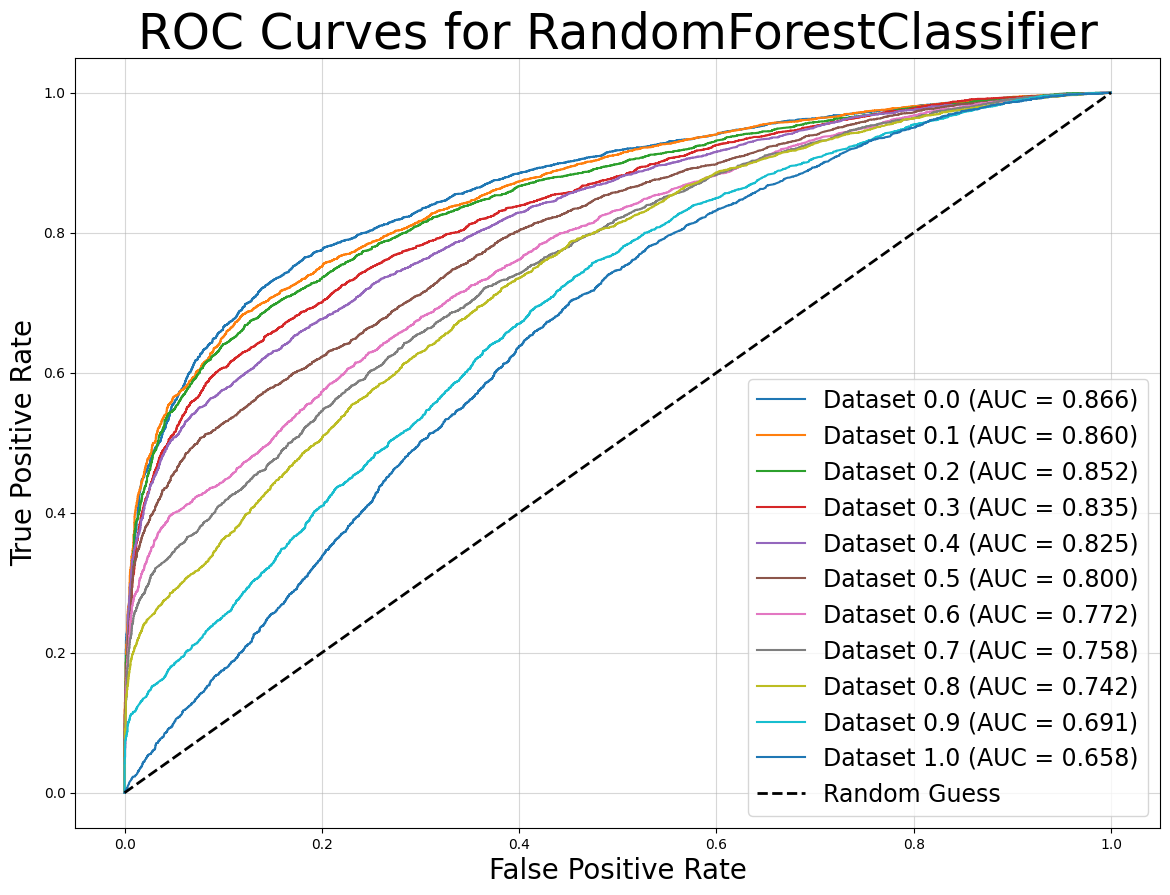
\includegraphics[width=\textwidth]{rf_auc.png}
            \end{figure}
        \end{column}
    \end{columns}

        \begin{footnotesize}
            \centering
            \textbf{Note:} We set \texttt{random\_state} to \texttt{0} for reproducibility.
        \end{footnotesize}
\end{frame}

\begin{frame}{Gradient Boosting}

    \textbf{Gradient Boosting} combines weak predictive models (in our case decision trees) in an iterative manner.

    \begin{columns}
        \begin{column}{0.45\textwidth}
            Each model corrects the errors of its predecessor, making it highly effective but sensitive to hyperparameter tuning.

            \vspace{-0.1em}

            {\small
            $$
            \begin{array}{|l|c|}
                \hline
                \textbf{Hyperparameter} & \textbf{Values} \\
                \hline
                \hline
                n\_estimators & 125 \\
                learning\_rate & 0.025 \\
                max\_depth & 3 \\
                subsample & 0.4 \\
                \hline
            \end{array}
            $$
            }
        \end{column}
            \begin{column}{0.55\textwidth}
                \begin{figure}
                    \centering
                    \vfill
                    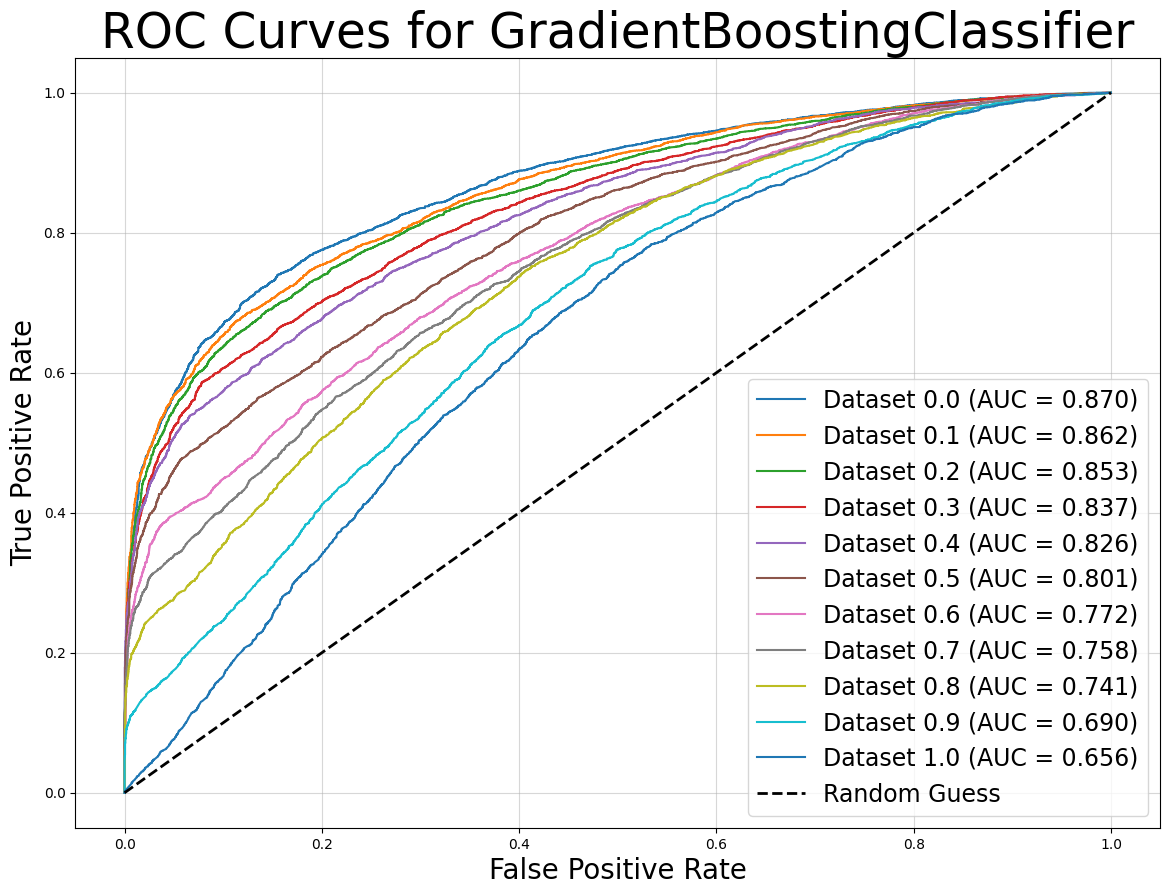
\includegraphics[width=\textwidth]{gbc_auc.png}
                \end{figure}
            \end{column}
    \end{columns}

\end{frame}

\begin{frame}{Extreme Gradient Boosting}

    \textbf{XGBoost} (\textit{Extreme Gradient Boosting}) is a scalable and efficient gradient boosting framework known for its regularization capabilities and speed.

    \vspace{-1em}

    \begin{columns}
        \begin{column}{0.45\textwidth}
            {\small
            $$
            \begin{array}{|l|c|}
                \hline
                \textbf{Hyperparameter} & \textbf{Values} \\
                \hline
                \hline
                n\_estimators & 100 \\
                learning\_rate & 0.1 \\
                max\_depth & 6 \\
                subsample & 0.7 \\
                gamma & 5 \\
                \hline
            \end{array}
            $$
            }
        \end{column}
        \begin{column}{0.55\textwidth}
            \begin{figure}
                \centering
                \vfill
                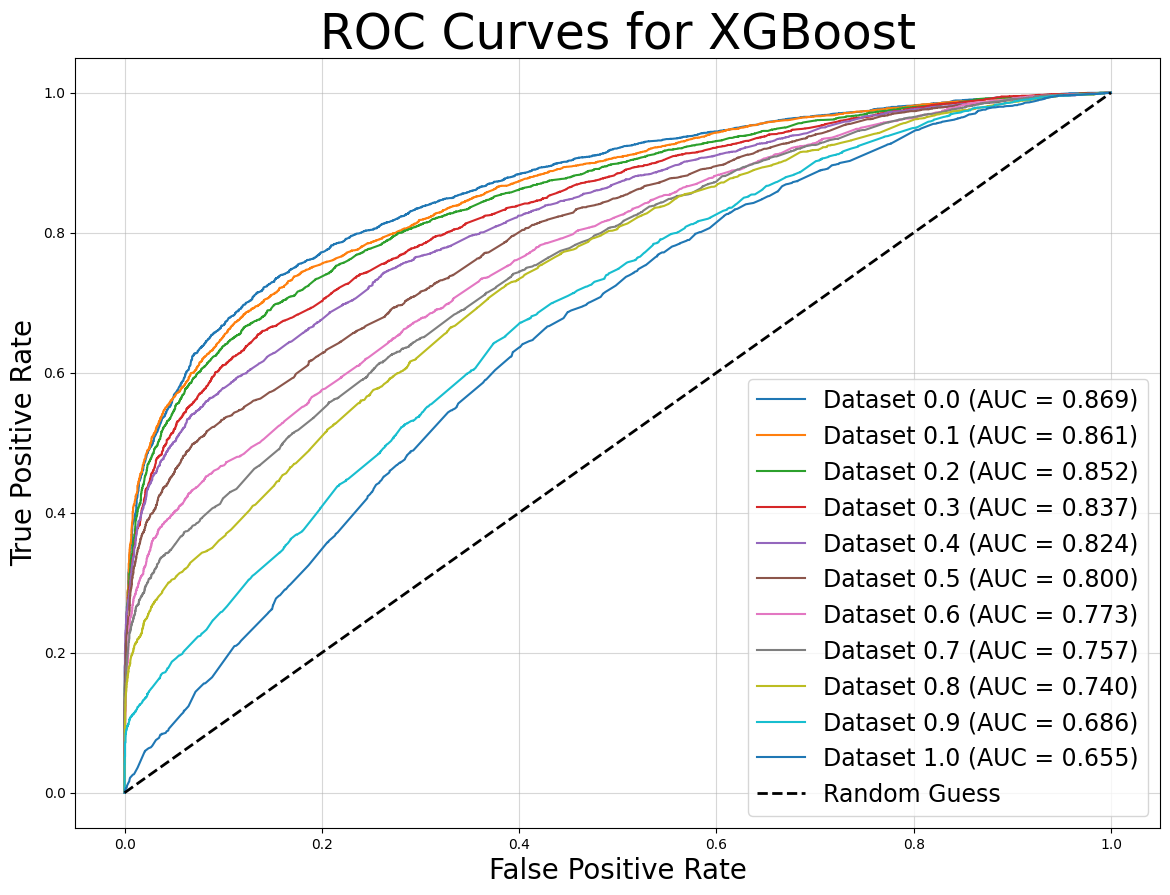
\includegraphics[width=\textwidth]{xgb_auc.png}
            \end{figure}
        \end{column}
    \end{columns}
\end{frame}

\begin{frame}{Performance Comparison}

    \begin{figure}
        \centering
        \vfill
        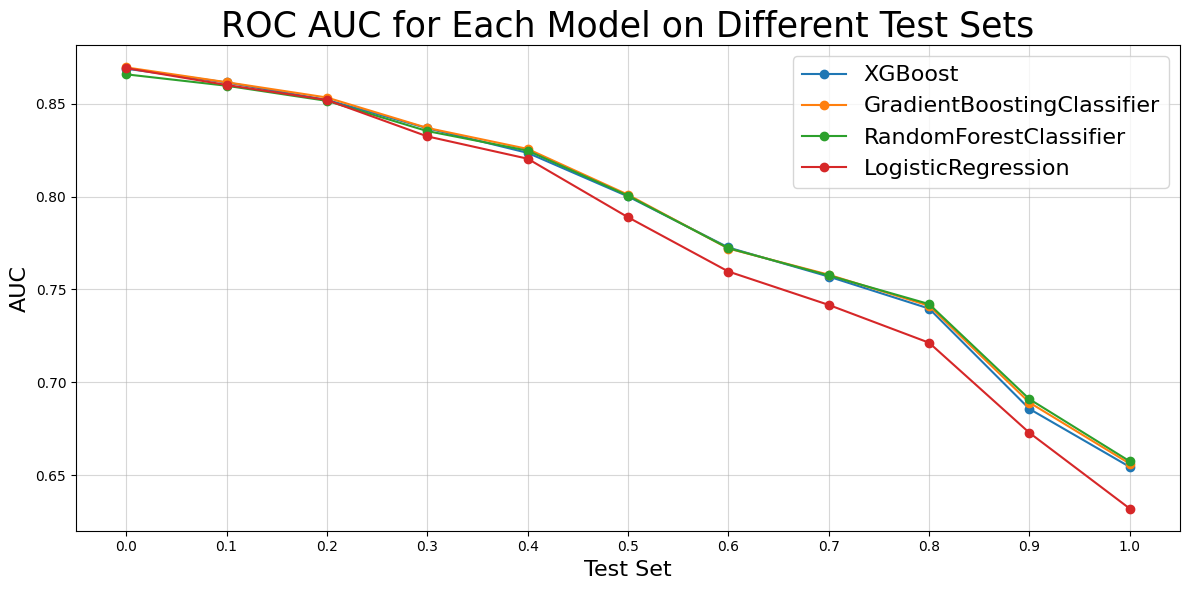
\includegraphics[width=\textwidth]{auc_comp.png}
    \end{figure}

\end{frame}

\begin{frame}{Statistical Performance Comparison}

    To give statistical support to our study we repeated this experiment $R = 50$ times. Keeping always the same training set (in order to not train the models several times), for each repetition we:
    \begin{enumerate}
        \item defined a new shifted ditribution $\mathcal{N}(\boldsymbol{\mu}_{\text{shift}}, \boldsymbol{\Sigma}_{\text{shift}}) $
        \item created 11 \textbf{testing} datasets $\mathcal{D}_\alpha$ with $\alpha \in \{0.0, 0.1, \ldots, 1.0\}$, where $\alpha$ represents the misture mixing probability
        \item computed the ROC-AUC score for each model on each testing dataset
    \end{enumerate}
\end{frame}

\begin{frame}{Statistical Performance Comparison}

    \begin{figure}
        \centering
        \vfill
        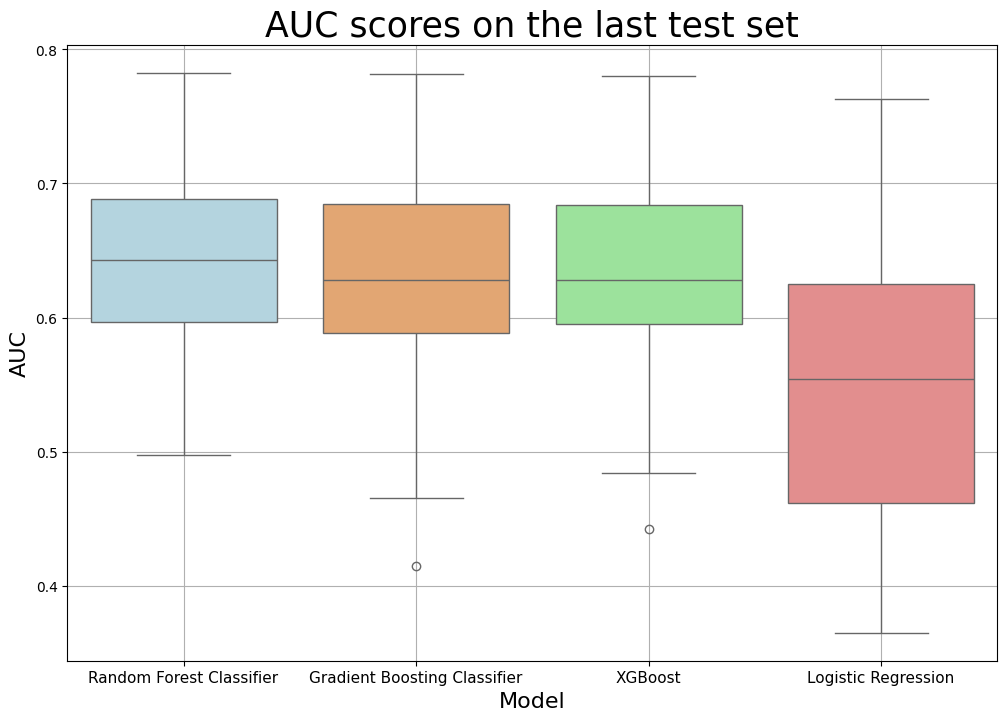
\includegraphics[width=0.8\textwidth]{boxplot.png}
    \end{figure}

\end{frame}
